\subsection{Mikroprocessor}
\subsubsection{Arduino Mega 2560}
For at kunne opfylde kriterierne sat i kravspecifikationen, er en Arduino Mega 2560 valgt. Denne besidder 256kb flash memory hvilket gør den mere brugbar i forhold til UCN boardet som har 128kb flash memory. \newline I takt med videreudvilking af produktet, anvedes et shield for at kunne anvende flere digitale pins. Da Ucn boardet ikke er kombatibelt med dette, ses dette som belæg for at anvende Arduino Mega. \newline
Mikroprocessoren besidder 54 digitale pins og 14 analog pins som fungerer som in- og output. Derudover har den 4 UART (hardware serial ports) pins som anvedes til at integrere med microproicessorens interface. Disse pins fungerer i et spændingsinterval på 0-5 V. \newline ATMega2560 som er Arduino Mega's processor har en clock frekvens på 16 MHz. Den kan få strøm gennem usb, power jack og gennem pin Vin og den anbefales en spænding mellem 7-12 V. \newline
Mikroprocessoren kan forbindes til computeren ved hjælp af usb som gør det muligt for de to enheder at kommunikere sammen. Gennem usb forbindelsen kan software overføres fra computeren. Om nødvendigt kan softwaren genstartes på mikroprocessoren gennem en resetknap som er monteret på dens PCB.\newline 
Arduino Mega har den fordel at være kombatibel med standard bibliotekerne fra Arduino hvorimod UCN boardet ville kræve at al software skal laves fra bunden.

\begin{figure}[h!]
  \centering
  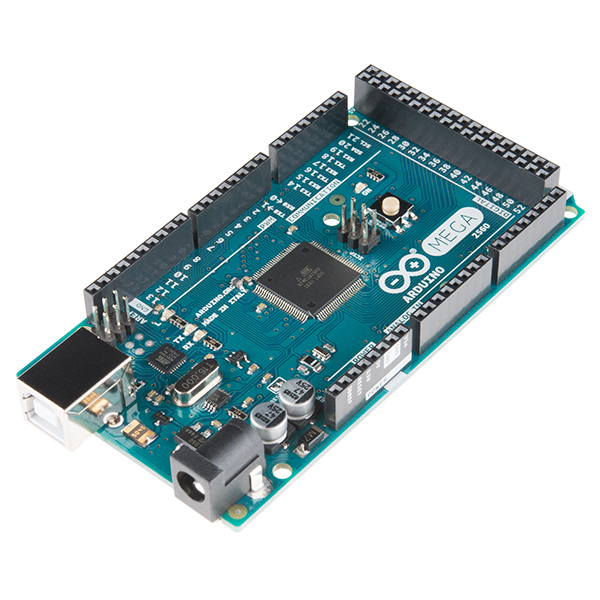
\includegraphics[width=0.7\textwidth]{figures/arduinoMega.jpg}
  \caption{Arduino Mega 2560.}
  \label{tempgraf_eksempel1}
\end{figure} 

\fxnote{fiks billede position}

\newpage



